\section{Le Bras Droit du Cruciverbiste (i.e. La Résolution de Mots Croisés)}

La troisième tâche est la résolution d'indices de mots croisés. Le concept est 
simple et ressemblent aux tâches précédentes dans son exploitation du réseau 
sémantique. Tandis que le chercheur de synonymes calcule la distance entre des 
mots individuels et le désambiguïseur trouve la distance entre deux séquences de 
mots, le resolveur de mots-croisés cherche la distance entre une séquence de 
mots (l'indice) et un mot (le mot cible). Comme précédemment, le noyau du 
programme est donc une recherche de la matrice de relations pour trouver un 
certain nombre de mots candidats. Par contre, des étapes supplémentaires sont 
nécessaires pour faire en sorte que les mot cibles adhèrent à certaines 
contraintes imposées par le jeu.

Le principe des mots croisés est de remplir une grille de lettres en fonction 
d'indices, de longueur de mots cibles et de caractères qui ont déjà été devinés 
dans la grille. Notre application est un outil support qui permet de fournir des 
mots candidats au cruciverbiste\footnote{Un amateur de mots croisés}. A part ces 
deux contraintes, il est important que les mots candidats correspondent à la 
catégorie syntaxique indiquée par l'indice. Notons que pour l'instant 
l'application ne détecte que les mots des catégories \lq{nom}\rq, \lq{adj}\rq, 
\lq{adv}\rq{} et \lq{verbe}\rq, puisque les autres catégories ne sont pas 
présentes dans le réseau. Par exemple, pour une indice \lq{escroqués}\rq, les 
mots candidats doivent être des participes passés qui sont conjugués au masculin 
pluriel, et pour une indice \lq{a l'air chouette}\rq, les mots candidats doivent 
être des verbes conjugués au troisème personne singulier du présent 
indicatif\footnote{Les bonnes réponses sont \lq{eus}\rq{}  et \lq{ulule}\rq{} 
respectivement}.

Le processus suivi est donc séquentiel et peut être représenté par le schéma 
suivant:

\begin{figure}[!ht]
\centering
\def\svgwidth{\columnwidth}
\input{crossword_schema.pdf_tex}
\caption{Le schéma du traitement pour la résolution des indices de mots croisés}
\label{fig:schema_crosswords}
\end{figure}

\subsection{Les étapes de traitement}
\subsubsection{Etape 1 : Identification de la catégorie syntaxique du mot cible}
Les indices sont de petites séquences de mots qui sont très rarement des phrases 
complètent et bien formées. Elles correspondent souvent à un syntagme 
particulier et contiennent parfois des ambiguïtés de catégorie syntaxique. Il 
est aussi possible à cette étape d'identifier quelques marques de flexion qui 
peuvent indiquer la forme du mot cible. Le réseau sémantique ne contient a 
priori ques des lemmes et donc il est important de garder ces indices 
flexionnelles pour reconjuguer les mots candidats à l'étape 3 [REF].  

Un étiqueteur syntaxique automatique tel que MElt[ 
\hyperref[bib:melt]{~\ref*{bib:melt}}] est peu adapté pour cette identification 
puisqu'il se base sur les probabilités pour renvoyer la séquence de tags la plus 
probable pour l'indice. Ceci signifie que le tag prédit peut ne pas correspondre 
à un des tags possibles pour un mot donné ou les ambiguïtés ne sont pas 
peut-être pas toutes reperées. De plus, de tels étiqueteurs sont dépendants de 
leurs données d'entraînement, et les indices des mots croisés sont d'une forme 
très différente des données du FTB sur lequel MElt a été entrainé. Nous 
choissisons donc de faire une analyse point à point des mots de l'indice afin de 
renvoyer toutes les possibilités catégorielles pour chaque mot. Le Lefff 
(Lexique des Formes Fléchies du 
Français)[\hyperref[bib:lefff]{~\ref*{bib:lefff}}] est utilisé pour retrouver 
toutes les catégories syntaxiques et marques flexionnelles de chaque mot. Cette 
méthode renvoie évidemment plus de catégories syntaxiques que souhaitées et crée 
de l'ambiguïté artificielle. Cependant, la précision des catégories renvoyées 
pour chaque mot est plus élevée et globalement le rappel est très élevé pour la 
séquence de mots. [EXPLAIN]

La catégorie cible peut être identifiée à partir de ces ensembles de catégories 
grâce à la régularité des formes des indices. Si une indice contient un seul 
mot, les catégories cibles sont celles du mot de l'indice. Sinon, la catégorie 
dépend en grande partie des premiers mots de l'indice. Par exemple, si une 
indice commence par un nom, ou une séquence \lq{det nom}\rq{} ou une séquence 
\lq{det adj nom}\rq{}, la catégorie cible, étant donné qu'il n'y a pas 
d'ambiguïté catégorielle serait, serait un nom. Dans certains cas, il est aussi 
possible d'identifier quel mot de l'indice indique la conjugaison du mot cible. 
Cette identification se fait à l'aide d'une mini-grammaire de seulement 14 
règles, qui sont reproduites ci-dessous :

\begin{framed}
det nc -\textgreater 2, nc\newline
det adj nc -\textgreater 3, nc\newline
adj nc -\textgreater 2, nc\newline
nc -\textgreater 1, nc\newline
adj prep -\textgreater 1, adj\newline
adv v -\textgreater 2, v\newline
advm v -\textgreater 2, v\newline
advneg v -\textgreater 2, v\newline
advneg advneg v -\textgreater 3, v\newline
v -\textgreater 1, v\newline
clr v -\textgreater 2, v\newline
prel v -\textgreater 2, adj \newline
cln v -\textgreater 2, n\newline
prep nc -\textgreater ?, adj
\end{framed}

Chaque ligne représente une règle différente. A gauche de la flèche est la 
séquence de mots qui indiquent, au début d'une indice, une certaine catégorie 
syntaxique. A droite de la flèche est l'indice (à partir de 1) du mot de la 
partie gauche dont les informations grammaticales seront utilisés pour conjuguer 
les mots cibles, et ensuite est la catégorie syntaxique du mot cible. 

Le jeu d'étiquettes utilisées est celle du Lefff\footnote{Ce jeu a été réduit 
pour ne contenir que les noms, adjectifs, adverbes et verbes}, qui est utilisée 
pour retrouver les formes fléchies. Une même indice peut correspondre à 
plusieurs règles différentes si un mot donné est ambigu pour la catégorie 
syntaxique.

Les catégories syntaxiques sont retenues pour le parcours du réseau et les 
informations grammaticales pour retrouver les formes fléchies correspondant aux 
lemmes trouvés dans le réseau.

Une particularité des indices est que parfois elles peuvent contenir plusieurs 
parties, séparées d'une virgule et qui représentent plusieurs sous-indices à 
l'intérieur de l'indice. Par exemple, une indice peut avoir la forme 
\lq{habillée, fringuée}\rq{} et dans ce cas, il est souhaitable de séparer cette 
indice en \lq{habillée}\rq{} et \lq{fringuée}\rq{} afin d'avoir la meilleur 
chance de trouver la catégorie voulue. Idéalement, ces deux parties devraient 
aussi correspondre en termes de catégorie syntaxique, ce qui signifie qu'il 
faudrait en théorie ne garder que les catégories cibles qui correspondent aux 
deux parties de l'indice. Par contre, nous optons pour le choix de garder toutes 
les catégories potentielles à partir des deux parties de l'indice pour nous 
assurer de la couverture maximale. 

\subsubsection{Etape 2 : Recherche du graphe}

A partir des lemmes trouvés dans le Lefff pour chaque mot de l'indice, et à 
partir de formes fléchies si les mots ne s'y trouvent pas\footnote{Même si le 
réseau ne devraient pas contenir de formes fléchies, il est possible qu'il en 
contient à cause des erreurs de tagging, et donc nous exploitons cette faiblesse 
ici pour augmenter la chance de retrouver le plus de mots de l'indice 
possibles.}, un vecteur de mots avec leur distance est obtenu pour représenter 
toute l'indice. Ce vecteur contient la moyenne des vecteurs des vingt plus 
proches voisins obtenus pour chaque mot dans un parcours du réseau. Cette 
moyenne permet de calculer les mots les plus proches de l'indice en général. Les 
catégories de mots recherchés sont les catégories obtenues à partir des règles 
de la mini-grammaire. Dans le cas où aucun règle correspond à l'indice, 
notamment dans le cas où un des premiers mots de l'indice ne se trouve pas dans 
le lexique, les mots recherchés sont de n'importe quelle catégorie.

\subsubsection{Etape 3 : Conjugaison des lemmes obtenus}

Les résultats de la recherche du graphe sont des lemmes, qui sont à modifier 
pour correspondre à la forme du mot recherché. En utilisant l'ensemble de 
catégories et d'informations grammaticales obtenues lors de l'étape 1 [REF], 
cette étape cherche les formes fléchies correspondantes à chaque lemme et 
vérifie lesquelles correspondent aux informations grammaticales recherchées pour 
les mots candidats.

\subsubsection{Etape 4 : Filtrage selon les contraintes}

La dernière étape filtre les candidates conjugués afin de ne renvoyer que les 
candidats qui se conforment aux contraintes de longueur de mot et de caractères 
déjà devinés. Il n'est pas possible de faire cette étape avant la conjugaison, 
puisque la conjugaison des lemmes peut avoir pour effet un changement dans la 
longueur du mot et des caractères qui y apparaîssent.

Souvent dans les outils d'aide de résolution de mots fléchés, cette étape est 
la seule incluse dans le programme, et donc un grand nombre de mots 
correspondent aux contraintes de longueur et de caractères. Dans notre 
programme, cette étape sert à enlever la grande quantité de bruit dans les 
résultats produits directement à partir du réseau, et permet de raffiner en 
grande partie les résultats. L'avantage d'utiliser le réseau et qu'il y a plus 
de chance d'avoir des résultats qui correspondent à l'indice donnée et non pas 
des mots candidats indépendant de l'indice, ce qui permet un traitement plus 
sophistiqué à cette étape.

\subsection{L'interface graphique}

L'interface graphique, implementée en python en utilisant les bibliothèques 
Tkinter [REF] et PMW [REF] sert à visualiser les résultats renvoyés aux 
différentes étapes du processus. Elle est mi-chemin entre un outil pour un 
joueur de mots croisés, qui ne s'intéresse que aux mots qui se conforment aux 
contraintes données et un outil plus pédagogue pour montrer les étapes de 
traitement.

\begin{center}
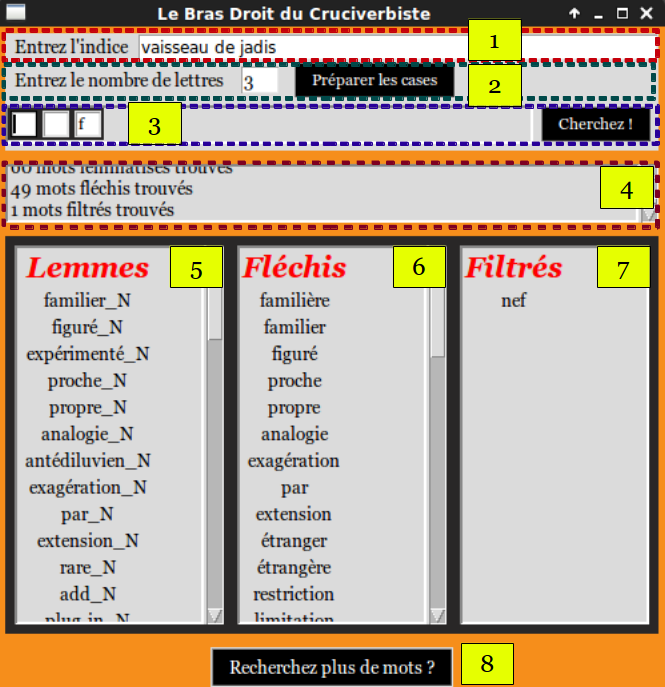
\includegraphics{CrossWordInterface.png}
\end{center}

\begin{enumerate}
    \item{L'indice qui sert à deviner le mot recherché}
    \item{Le nombre de lettres du mot recherché. En cliquant sur \lq{Préparer l
    es cases}\rq, cette contrainte sera enregistrée et les cases générées en 3.}
    \item{Les cases pour entrer les caractères déjà devinés. Cette contrainte 
    sera prise en compte dans le filtrage des mots candidats}
    \item{Le log qui permet de tracer le suivi du programme. Ici seront 
    affichés des avertissements dans le cas où un mot n'est pas reconnu, la/les 
    catégorie(s) syntaxique(s) du mot recherché et le nombre de résultats 
    renvoyés à chaque tour.}
    \item{Les plus proches voisins de l'indice. Au départ les vingt mots les 
    plus proches seront retournés.}
    \item{Les formes fléchies des lemmes renvoyés en 5., qui devraient 
    correspondre aux contraintes flexionnelles imposées par les mots de 
    l'indice, si elles sont reconnues}
    \item{Les candidats filtrés selon les contraint de longueur de mot et de 
    caractères déjà devinés.}
    \item{Si l'utilisateur veut continuer en regardant les vingt prochains plus 
    proches mots, il peut cliquer sur ce bouton pour renvoyer plus de 
    résultats. Ceci peut être utile dans le cas où peu de résultats fléchis ou 
    filtrés sont renvoyés.}
    
\end{enumerate}


\subsection{Evaluation}
Le système est difficilement évaluable contre d'autre systèmes de la même 
nature, parce qu'il n'existe pas de système d'évaluation standard et de scores 
comparatifs. Il existe beaucoup de systèmes qui ne se basent pas sur la 
similarité sémantique, mais qui renvoient plutôt tous les mots qui correspndent 
aux contraintes de longueur et de caractères déjà devinés, et ces systèmes ne 
fournissent pas un bon moyen de comparer l'approche par réseau sémantique.

Notre évaluation est donc une évaluation simple de la capacité du réseau de 
trouver la solution d'une indice, et qui compare le taux de réussite pour 
différents niveaux de difficulté et pour différentes catégories syntaxiques. 
L'évaluation se fait sur un petit corpus d'indices pris d'un site internet de 
mots fléchés [REF 
http://www.notretemps.com/jeux/jeux-en-ligne/mots-fleches-gratuits], qui classe 
les grilles par niveaux. Le corpus se trouve dans l'annexe [REF - put in 
annexe]. Il est vrai que l'emplacement des mots dans la grille les uns par 
rapport aux autres contribue au niveau global de la grille, mais nous estimons 
que le niveau est aussi reflété dans la difficulté des indices individuelles. Le 
corpus contient deux niveaux différents (1 et 2) et pour chaque niveau vingt 
noms communs, vingt noms propres, vingt adjectifs et vingt verbes. Les indices 
étaient prises aussi objectivement que possible, avec soin de ne pas répéter le 
même mot cible entre deux indices, ou de prendre exclusivement des indices qui 
contiennent une seule tournure. Autant de solutions de chaque catégorie ont été 
sélectionnées afin de comparer le taux de réussite pour chaque catégorie, mais 
le constat a été que le niveau contient plus de noms communs et moins de nom 
propres, ce qui influence aussi la difficulté des indices, et ceci sera pris en 
compte lors de l'analyse des résultats.

Etant donné que notre système est clairement orienté vers une optimisation du 
rappel, il est moins pertinent de le juger par rapport à la précision des 
résultats, même si un système idéal serait aussi précis. Pour chaque catégorie 
syntaxique, nous cherchons d'abord si la solution apparaît dans le réseau et si 
oui, après combien de voisins les plus proches le mot est trouvé. Pour éviter de 
parcourir tout le réseau en cas de non-découverte, nous limitons le maximum de 
voisins renvoyés à 100. Au délà de 100, le mot est considéré non-trouvé.





\subsection{Améliorations possibles}
